\documentclass{article}
\usepackage{nips10submit_e,times}
%\documentstyle[nips07submit_09,times]{article}
\usepackage[square,numbers]{natbib}
\usepackage{amsmath, epsfig}
\usepackage{amsfonts}
\usepackage{subfigure}
\usepackage{graphicx}
\usepackage{amsfonts}
\usepackage{algorithm}
\usepackage{algorithmic}
\usepackage{easybmat}
\usepackage{footmisc}
\renewcommand\algorithmiccomment[1]{// \textit{#1}}
%
\newcommand{\ignore}[1]{}
\newcommand{\comment}[1]{}
\DeclareMathOperator*{\argmax}{arg\,max}

\title{Probabilistic Deterministic Infinite Automata}


\author{
David Pfau \\
Center for Theoretical Neuroscience \\
Columbia University\\
New York, NY 10027, USA \\
\texttt{pfau@neurotheory.columbia.edu} \\
\AND
Nicholas Bartlett\thanks{ http://www.stat.columbia.edu/~bartlett} \\
Department of Statistics\\
Columbia University\\
New York, NY 10027, USA \\
\texttt{bartlett@stat.columbia.edu} \\
\And
Frank Wood \\
Department of Statistics\\
Columbia University\\
New York, NY 10027, USA \\
\texttt{fwood@stat.columbia.edu} \\
}

% The \author macro works with any number of authors. There are two commands
% used to separate the names and addresses of multiple authors: \And and \AND.
%
% Using \And between authors leaves it to \LaTeX{} to determine where to break
% the lines. Using \AND forces a linebreak at that point. So, if \LaTeX{}
% puts 3 of 4 authors names on the first line, and the last on the second
% line, try using \AND instead of \And before the third author name.

\newcommand{\fix}{\marginpar{FIX}}
\newcommand{\new}{\marginpar{NEW}}
\newcommand{\q}{\xi}
\newcommand{\state}{q}
\newcommand{\symb}{\sigma}
\newcommand{\bmu}{\boldsymbol\mu}
\newcommand{\bphi}{\boldsymbol\phi}
\newcommand{\bpi}{\boldsymbol\pi}

%\nipsfinalcopy

\begin{document}

\maketitle

% !TEX root = deplump.tex
\subsection*{Abstract}



% !TEX root = main.tex
\section{Introduction}
\label{section_introduction}

Predictive models are all about doing as much as you can with as little data and computation as possible.  If sufficient for application purposes, resorting to simple models is often effective.  

Richly expressive models require   

Bayesian approaches to prediction dictate tying and sharing parameters, often through hierarchies and so forth. 

Cite 

Related work on multiscale language modeling
\citep{Goldwater2009,Mochihashi2009}

Related work on transformed Dirchlet processes and HDP's with random effects.
\citep{Sudderth2005,Kim2007,Hoffman2009,}
\section{Probabilistic Deterministic Finite Automata}
A PDFA is formally defined as a 5-tuple $M = (Q,\Sigma,\delta,\pi,q_0)$.  $Q$ is a finite set of states. $\Sigma$ is a finite alphabet of observable symbols. $\delta\,:\,Q\times\Sigma\rightarrow Q$ is the transition function from a state/symbol pair to the next state.  $\pi\,:\,Q\times\Sigma\rightarrow[0,1]$ is the probability of the next symbol given a state.  $q_0$ is the initial state.  For clarity and minimal clutter, we use $i$ to index over elements of $Q$, $j$ to index over elements of $\Sigma$ and $t$ to index elements of an observed string.  For example, $\delta_{ij}$ is shorthand for $\delta(q_i,s_j)$.

The odd-sounding ``probabilistic deterministic" refers to the fact that a string of symbols is generated by a two-stage process.  Given a state $q_i$, the probability that the next symbol is $s$ is given by $\pi(q_i,s)$, hence ``probabilistic."  We denote the multinomial distribution over symbols given a state $q_i$ as $\pi_i$, so we could equivalently say $s \sim \pi_i$.  Given a state $q_i$ and a symbol $s$, however, there is a {\it unique} state $\delta(q_i,s)$ that follows it, hence ``deterministic."  

We can see that n-grams or nth-order Markov models are a particular class of PDFAs.  If we consider a state to be the prefix $x_1 x_2 \ldots x_{n-1}$, then given a state and a symbol $x_n$, the unique next state is $x_2 \ldots x_n$.  Thus nth-order Markov models are a subclass of PDFAs with $|\Sigma|^n$ states.

PDFAs themselves are a subclass of hidden Markov models (HMMs).  Specifically, they are the class of HMMs for which, given a sequence of observed data, there is only one possible path through the hidden states.  Our approach to inference, taking posterior samples over the space of models, while forcing the path through these models to be deterministic, can be seen as an extreme case of the tradeoff inherent in most model learning.  Normally, one has to estimate both the model and the parameters of the model, but in this case all of the uncertainty is shifted onto the model itself.

\section{Bayesian PDFA Inference}

The outline of this section is as follows.  We define a prior distribution over PDFAs with a fixed number of states and show that many of the parameters can be integrated out.  We derive a Metropolis-Hastings sampler for posterior inference in the finite model, and show that many of the elements of the transition matrix can be ignored without affecting the correctness of sampling.  We then let the number of states go to infinity and show that the limit is well defined.  This is the probabilistic deterministic infinite automaton (PDIA).  Inference in the PDIA carries over from the finite case in a natural way.

\subsection{A Prior over PDFAs}

We assume that the states $Q$, alphabet $\Sigma$ and initial state $q_0$ are known, and define a prior over the transition function $\delta$ and emission probabilities $\pi$.  In the finite case $\delta$ and $\pi$ can be thought of as matrices, with columns indexing elements of $\Sigma$ and rows indexing elements of $Q$.  For each column $j$ of the transition matrix $\delta$, we sample the rows i.i.d. from a discrete distribution $\bphi_j$ over $Q$, that is, $\delta \sim [\bphi_1\ldots\bphi_{|\Sigma|}]$.  The $\bphi_j$ themselves are sampled i.i.d. from a Dirichlet prior with parameters $\alpha\bmu$, where $\alpha$ is a concentration and $\bmu$ is itself drawn from a uniform Dirichlet distribution, with $\gamma$ total pseudocounts.  This hierarchical Dirichlet construction allows elements of $\delta$ to be coupled together in a way that remains well-behaved in the limit of infinite states.  We also place a uniform Dirichlet prior over the per-state emission probabilities $\bpi_i$ with $\beta$ total pseudocounts.  Formally:

\begin{eqnarray}
\bmu|\gamma,|Q| & \sim & \mathrm{Dir}\left(\gamma/|Q|,\ldots,\gamma/|Q|\right) \label{gen:mu} \\
\bphi_{j}|\alpha,\bmu  & \sim & \mathrm{Dir}(\alpha\bmu) \label{gen:phi} \\
\bpi_{i}|\beta,|\Sigma| & \sim & \mathrm{Dir}(\beta/|\Sigma|,\ldots,\beta/|\Sigma|) \label{gen:pi}\\
\delta_{ij} & \sim & \bphi_{j} \label{gen:delta}
\end{eqnarray}

where $i$ goes from 0 to $|Q|-1$ and $j$ goes from 1 to $|\Sigma|$.  From this we generate a sequence of $T$ symbols:

\begin{eqnarray}
\q_0 & = & q_0 \label{gen:q0} \\
x_0 & \sim & \bpi_0 \label{gen:x0} \\
\q_t & = & \delta(\q_{t-1},x_{t-1}) \label{gen:q} \\
x_t & \sim & \bpi_t \label{gen:x}
\end{eqnarray}

We choose this particular inductive bias, with transitions tied together within a column of $\delta$, because the most recent symbol ought to be informative about what the next state is.  If we instead had a single Dirichlet prior over all elements of $\delta$, transitions to a few states would be highly likely no matter the context and those states would dominate the behavior of the automata.  If we tied together rows of $\delta$ instead of columns, being in a particular state would tell us more about the sequence of states we came from than the symbols that got us there.  As we would like states to be good statistics of the past for predicting the future, a bias that depends on the most recent symbol is preferable.

Given data, the likelihood is

\[ p(x_{0:T}|\delta,\pi) = \pi(\q_0,x_0)\prod_{t=1}^T \pi(\q_t,x_t) \label{x:def} \]

We can marginalize out $\pi$ and express the likelihood in a form that depends only on the counts of symbols emitted from each state.  Define the count matrix $c$ for the sequence $x_{0:T}$ and transition matrix $\delta$ as $c_{ij} = \displaystyle\sum_{t=0}^T I_{ij}(\q_t,x_t)$, where $I_{ij}(\q_t,x_t)$ is an indicator function that is 1 if $\q_t = q_i$ and $x_t = \sigma_j$, 0 otherwise. This matrix gives the number of times each symbol is emitted from each state.  Thanks to multinomial-Dirichlet conjugacy we can integrate out $\pi$ and express the probability of a sequence given the transition function $\delta$ solely in terms of $c$ and $\beta$:

\begin{eqnarray}
 p(x_{0:T}|\delta,\beta) & = & \int p(x_{0:T}|\pi,\delta) p(\pi|\beta) d\pi \label{x:factor} \\
 & = &  \prod_{i=0}^{|Q|-1} \frac{\Gamma(\beta)}{\Gamma(\frac{\beta}{|\Sigma|})^{|\Sigma|}} \int\pi_{i1}^{\frac{\beta}{|\Sigma|}+c_{i1}-1} \pi_{i2}^{\frac{\beta}{|\Sigma|}+c_{i2}-1} \ldots \pi_{i|\Sigma|}^{\frac{\beta}{|\Sigma|}+c_{i|\Sigma|}-1} d\bpi_i \label{x:int}\\
 & = & \prod_{i=0}^{|Q|-1} \frac{\Gamma(\beta)}{\Gamma(\frac{\beta}{|\Sigma|})^{|\Sigma|}} \frac{\prod_{j=1}^{|\Sigma|}\Gamma(\frac{\beta}{|\Sigma|} + c_{ij})}{\Gamma(\beta + \sum_{j=1}^{|\Sigma|} c_{ij})} \label{x:end}
 \end{eqnarray}
 
 The dependence of $c$ on $\delta$ is only through $\q_{0:T}$, and changing a single element of $\delta$ can have a complex effect on $c$.  By changing a single transition $\delta_{ij}$, all states downstream of the first time $q_i$ emits $\sigma_j$ are affected, and some elements of $c$ that were zero may become nonzero, and vice versa.
 
 The likelihood of a particular transition matrix $\delta$ given $\bmu$ has a similar form.  Let $v_{ij}$ be the number of times that $\delta_{i'j} = q_i$ for all $i'$ in the column $j$, that is, $v_{ij} = \displaystyle\sum_{i' = 0}^{|Q|-1} I_{i}(\delta_{i'j})$, $I_i(q_{i'})$ being the indicator function that is only 1 when $q_i' = q_i$.  Given $\bmu$, we can integrate out $\phi$ and express the likelihood of $\delta$ in terms of $\bmu$:
 
 \begin{eqnarray}
 p(\delta|\bmu,\alpha) & = & \int p(\delta|\phi)p(\phi|\bmu,\alpha) d\phi \label{delta:factor}\\
  & = & \prod_{j=1}^{|\Sigma|} \frac{\Gamma(\alpha)}{\prod_{i=0}^{|Q|-1}\Gamma(\alpha\mu_i)} \int \phi_{0j}^{\alpha\mu_0+v_{0j}-1} \phi_{1j}^{\alpha\mu_1+v_{1j}-1} \ldots \phi_{|Q|-1,j}^{\alpha\mu_{|Q|-1}+v_{|Q|-1,j}-1} d\bphi_j \label{delta:int}\\
  & = &  \prod_{j=1}^{|\Sigma|} \frac{\Gamma(\alpha)}{\prod_{i=0}^{|Q|-1}\Gamma(\alpha\mu_i)} \frac{\prod_{i=0}^{|Q|-1} \Gamma(\alpha\mu_i + v_{ij})}{\Gamma(\alpha + |Q|)} \label{delta:end}
  \end{eqnarray}

%Finally, the posterior probability of $\bmu$ given $\delta$ is

%\begin{eqnarray}
%p(\bmu|\delta,\alpha, \gamma) & = & \frac{p(\delta|\bmu,\alpha)p(\bmu|\gamma)}{\int p(\delta|\bmu,\alpha)p(\bmu|\gamma) d\bmu}
%\end{eqnarray}

These are the ingredients we need for posterior inference.
 
 \subsection{Posterior Inference in the Finite Model}
 
We perform posterior inference in the finite model by Gibbs sampling elements of $\delta$ and the vector $\bmu$.  From the formulas above, it is straightforward to write down the conditional probability for one element of the transition matrix $\delta$.  If $\delta_{ij}$ is the element we are sampling, and $\delta_{-ij}$ is the rest of the matrix, with $\delta_{ij}$ removed, then

\begin{equation}
p(\delta_{ij}|\delta_{-ij},x_{0:T},\bmu,\alpha) \propto p(x_{0:T}|\delta_{ij},\delta_{-ij})p(\delta_{ij}|\delta_{-ij},\bmu,\alpha) \label{delta:cond}
\end{equation}

Both terms on the right hand side of this equation have closed-form expressions, the first given in \eqref{x:end}.  The second can be found from \eqref{delta:end} to be

\begin{equation}
P(\delta_{ij} = q_{i'}|\delta_{-ij},\alpha,\bmu) = \frac{\alpha\mu_{i'} + v_{i'j}}{\alpha + |Q| - 1} \label{delta:pred}
\end{equation}

Where $v_{i'j}$ is the number of elements in column $j$ equal to $q_{i'}$ {\em excluding} $\delta_{ij}$.  As $|Q|$ is finite, we can construct and normalize the conditional probability vector for $\delta_{ij}$ and sample.

We can simplify inference by ignoring transitions $\delta_{ij}$ for which the corresponding count $c_{ij}$ are 0.  Note that the likelihood of the data on the right hand side of \eqref{delta:cond} does not depend on $\delta_{ij}$ if $c_{ij} = 0$, so sampling conditioned on the data is the same as sampling without conditioning on the data.  Thus, if changing some other transition means $c_ij$ becomes 0, we can remove $\delta_{ij}$ until another transition is changed so the count again is nonzero, and we sample a new value for $\delta_{ij}$ from \eqref{delta:pred}, just as we would have during Gibbs sampling had we not removed it.  Note that the joint distribution over a column of $\delta$ is exchangeable, and so removing an observation is the same as marginalizing it out, meaning that sampling the other elements of $\delta$ is still correct, but now conditioned on the model where superfluous transitions are marginalized out.  When we remove multiple elements from a column of $\delta$, we have to replace the $|Q| - 1$ in the denominator of \eqref{delta:pred} with $K^+_j = \sum_{i=0}^{|Q|-1}v_{ij} \leq |Q|$, the number of entries in the $j$th column of $\delta$ that are {\em not} marginalized out.

The posterior for $\bmu$ up to a normalization constant is

\begin{eqnarray}
p(\bmu|\delta,\alpha,\gamma) & \propto & p(\bmu|\gamma) p(\delta|\bmu,\alpha)\nonumber \\
& = & \frac{\Gamma(\gamma)}{\Gamma(\frac{\gamma}{|Q|})^{|Q|}}(\mu_1\ldots\mu_{|Q|})^{\frac{\gamma}{|Q|}-1}\prod_{j=1}^{|\Sigma|} \frac{\Gamma(\alpha)}{\prod_{i=0}^{|Q|-1}\Gamma(\alpha\mu_i)} \frac{\prod_{i=0}^{|Q|-1} \Gamma(\alpha\mu_i + v_{ij})}{\Gamma(\alpha + K^+_j)}
\end{eqnarray}

We can sample this by Metropolis-Hastings, for example using Dir($\eta\hat\bmu$) as the proposal, where $\hat\bmu$ is our current estimate and $\eta$ is a large concentration parameter, or take the MAP estimate as in \cite{Mackay1995}.  Fortunately in the infinite limit a more natural way to sample presents itself.
 
 \subsection{The Probabilistic Deterministic Infinite Automaton}
 
 We now consider what happens when $|Q|\rightarrow\infty$.  Given a finite amount of data, there can only be nonzero counts for a finite number of state/symbol pairs, so we can marginalize out all but at most $T$ elements of $\delta$.  Denote these active entries by $\delta^T$.  The predictive probability for a new $\delta_{ij} = q_{i'}$ given $\delta^T$ is given by $\frac{\alpha\mu_{i'} + v_{i'j}}{\alpha + K^+_j}$.  Note that this only depends on $|Q|$ through $\mu_{i'}$, which is well behaved as $|Q|$ grows.  In the limiting case, most of the mass of $\bmu$ will concentrate on a handful of elements, and $\bmu$ becomes a draw from a {\em Dirichlet process} (DP), which is commonly used as a prior in Bayesian models with infinite parameters.  The hierarchical Dirichlet construction given in \eqref{gen:mu} and \eqref{gen:phi} becomes a {\em hierarchical Dirichlet process} (HDP), where the $\bphi_j$ are draws from a Dirichlet process whose parameters are given by $\alpha$ and $\bmu$, which is itself a draw from a Dirichlet process.  An attractive property of HDPs is that both the $\bphi_j$ and $\bmu$ can be integrated out, which makes sampling more straightforward than in the finite case.  This  representation of the model, with all draws from a DP integrated out, is known as the {\em Chinese Restaurant Franchise} (CRF).  This curious name needs some explanation, which we happily provide.
 
%We can sample incrementally from the joint distribution over $x_{0:T}$ and $\delta$ when $\phi_j$, $\mu$ and $\pi_i$ are integrated out in the $|Q|\rightarrow\infty$ limit.  From the start state $q_0$, we sample a symbol $s_{j_0}$ uniformly and assign $\delta_{0j_0}$ to a new state.  If $q^t = q_i$ then $x_t$ has the probability

% \[P(x_t=s_j|q_i,x_{0:t-1},q^{0:t-1}) = \frac{c_{ij}+\frac{\beta}{|\Sigma|}}{c_{i\cdot} + \beta}\]
 
% where $c_{ij}$ is the number of times so far $s_j$ was emitted from $q_i$ and $c_{i\cdot}$ is the total number of times $q_i$ has been visited so far.  
 
%If the state/symbol pair $(q_i,s_j)$ has not been visited before, we have to sample $\delta_{ij}$.  The two-stage generative procedure for elements of $\delta$ means that we have to keep track of counts at two levels.  Each $\delta_{ij}$ belongs to a cluster $v_{kj}$ that contains other $\delta_{i'j}$, while each $v_{kj}$ belongs to a top-level cluster $w_{l}$ that has elements across all $j$.  Each top level cluster has one $q \in Q$ assigned to it, and $\delta_{ij}$ is equal to that $q$ in the top cluster that the cluster with $\delta_{ij}$ belongs to (*might want to make this part clearer...add a figure*).  Let $\delta^t$ denote the elements of $\delta$ that have been visited at time $t$.  as follows:
 
%\[P(\delta_{ij} = k|\delta^t) \propto \begin{cases} & if $k \leq |\delta^t|$ \cr  & if $k > |\delta^t|$ \end{cases}\]
 
% This process for sampling from an HDP when $\mu$ and $\phi_j$ are integrated out is known as the {\em Chinese Restaurant Franchise Process}.

% \section{Posterior Inference over PDFAs}
 
 We perform posterior inference by sampling assignments for $\delta_{ij}$ individually.  Rather than ordinary Gibbs sampling, we use a mixed Gibbs/Metropolis-Hastings update.  To see why, consider the following case:  $\delta_{ij}$ is the only sampled element of $\delta$ that is assigned to the state $q_{i'}$.  When we removed $\delta_{ij}$ from the counts to sample it, the probability of assigning it back to $q_{i'}$ becomes zero, and even if it is assigned to some new state $q_{i''}$, the probability that $\delta_{i'j} = \delta_{i''j}$ for all $j$ visited by the data is low.  We do not want to forget a good sample, so instead we propose a new $\delta_{ij}$ and accept or reject according to the usual Metropolis-Hastings ratio.
 
Samples from the CRF are exchangeable, so we can remove $\delta_{ij}$ and propose a sample $\delta{ij}^*$ according to the CRF given $\delta_{-ij}^T$, the elements of $\delta$ visited by $x_{0:T}$ excluding $\delta_{ij}$.  This is the prior probability excluding the data, which cancels with the equivalent term in the posterior, meaning that the accept probability $\alpha(\delta_{ij},\delta_{ij}^*)$ is given by the ratio of the likelihood of the data

\[ \alpha(\delta_{ij},\delta_{ij}^*) =  \mathrm{min}\left(1,\frac{p(x_{0:T}|\delta_{ij}^*,\delta_{-ij}^T)}{p(x_{0:T}|\delta_{ij},\delta_{-ij}^T)}\right)\]

In general the numerator cannot be evaluated because changing $\delta_{ij}$ means changing the entire sequence of states visited by the data after $\delta_{ij}$ is first visited.  In practice we estimate the numerator by Monte Carlo approximation, sampling elements of $\delta$ according to the CRF as they are first visited by the data.  Changing one element of $\delta$ means many already-sampled state/symbol pairs may never be visited by the data, and have no effect on the likelihood.  The posterior probability of any value for these elements of $\delta$ is the same as the prior, and therefore we may remove them from $\delta^T$ after accepting a new $\delta_{ij}$.

% !TEX root = main.tex
\section{Theory and Related Work}
\label{sec:theory}

The PDIA posterior distribution takes the form of an infinite mixture of PDFAs.  In practice, we run a sampler for some number of iterations and approximate the posterior with a finite mixture of PDFAs.  For this reason, we now consider the expressive power of finite mixtures of PDFAs.  We show that they are strictly more expressive than PDFAs, but strictly less expressive than hidden Markov models.
%
%The natural generalization of PDFAs is to probabilistic {\em non}-deterministic finite automata (PNFA), which are like PDFAs except the transition function $\delta$ is stochastic.  That is, given a state and a symbol emitted from that state, the next state is chosen from distribution over successor states.  \comment{If all successor state distributions assign mass to only one state, the PNFA is a PDFA.}  PNFAs have the same expressive power as hidden Markov models: for any HMM there is a PNFA that defines the same distribution over strings, and vice versa \cite{Dupont2005}.
%
\begin{figure}[htbp]
\begin{center}
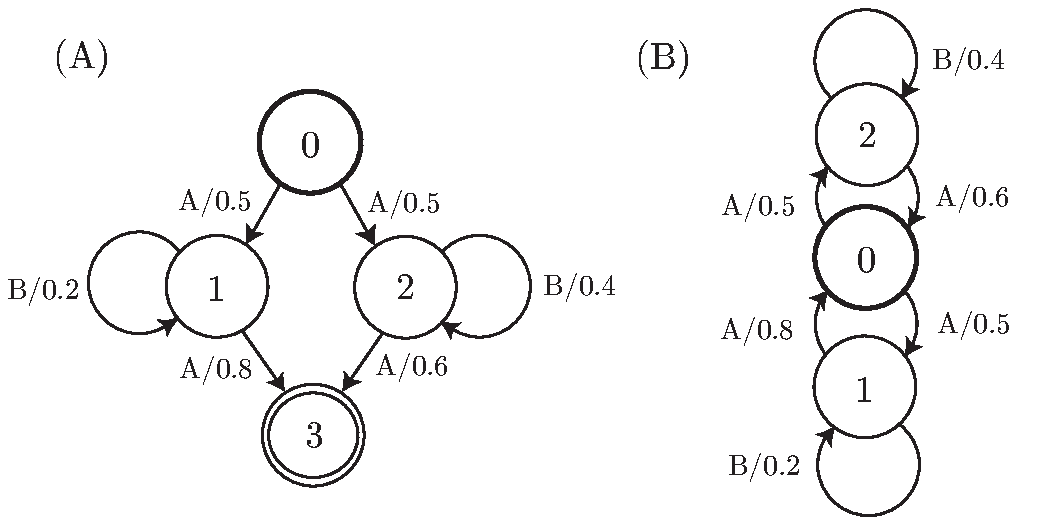
\includegraphics[scale=0.4]{pnfa.pdf}
\caption{Two PNFAs outside the class of PDFAs.  (a) can be represented by a mixture of two PDFAs, one following the right branch from state 0, the other following the left branch.  (b), in contrast, cannot be represented by any finite mixture of PDFAs.}
\label{pnfa}
\end{center}
\end{figure}
%
Probabilistic {\em non}-deterministic finite automata (PNFA) are a strictly larger model class than PDFAs.  For example, the PNFA in \ref{pnfa}(a) cannot be expressed as a PDFA.  However, it can be expressed as a mixture of two PDFAs, one with $Q = \{q_0,q_1,q_3\}$ and the other with $Q = \{q_0,q_2,q_3\}$.  Thus mixtures of PDFAs are a strictly larger model class than PDFAs.  In general, any PNFA where the nondeterministic transitions can only be visited once can be expressed as a mixture of PDFAs.  However, if we replace transitions to $q_3$ with transitions to $q_0$, as in \ref{pnfa}(b), there is no longer any equivalent finite mixture of PDFAs, since the nondeterministic branch from $q_0$ can be visited an arbitrary number of times.    \comment{This can be done by splitting a PNFA with $n$ possible values for $\delta(q_i,s_j)$ into $n$ PNFAs with deterministic $\delta(q_i,s_j)$, and repeating until all transitions are deterministic.  This includes the class of acyclic PNFAs as a trivial subset.  If there are any cycles that return to a state with nondeterministic transition, there is no equivalent finite mixture of PDFAs.}
%
\comment{It is important to note that the algorithm presented here will not always discover the appropriate mixture of PDFAs if the data-generating mechanism is like that in \ref{pnfa}(a).  Our intent is to clarify where the class of models that includes our posterior estimate falls in the Chomsky hierarchy, rather than to make any claim as to what class of models can be efficiently learned.}

Previous work on PDFA induction has focused on accurately discovering model structure when the true generative mechanism is a PDFA.  State merging algorithms do this by starting with the trivial PDFA that only accepts the training data and merging states that pass a similarity test \cite{Carrasco1994,Thollard2000}, and have been proven to identify the correct model in the limit of infinite data.  State splitting algorithms start at the opposite extreme, with the trivial single-state PDFA, and split states that pass a difference test \cite{Ron1996,Shalizi2004}.  These algorithms return only a deterministic estimate, while ours naturally expresses uncertainty about the learned model.

To test if we can learn the generative mechanism given our inductive bias, we trained the PDIA on data from three synthetic grammars: the even process \cite{Shalizi2004}, the Reber grammar \cite{Reber1967} and the Feldman grammar \cite{Feldman1966}, which have up to 7 states and 7 symbols in the alphabet.  In each case the mean number of states discovered by the model approached the correct number as more data was used in training.  Results are presented in Figure~ \ref{fig:synthetic_grammar_and_synth_results}.  Furthermore, the predictive performance of the PDIA was nearly equivalent to the actual data generating mechanism.  Details are given in the appendix.
%
\begin{figure}[htbp]
\centering
\subfigure[Even]{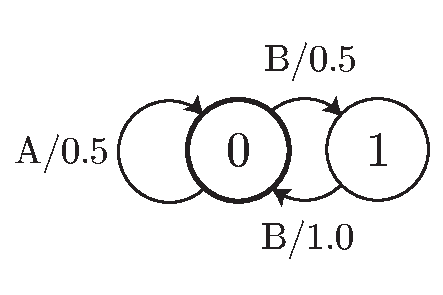
\includegraphics[scale=0.32]{even.pdf}\label{subfig:even}} \hspace{-.55cm} 
\subfigure[Reber]{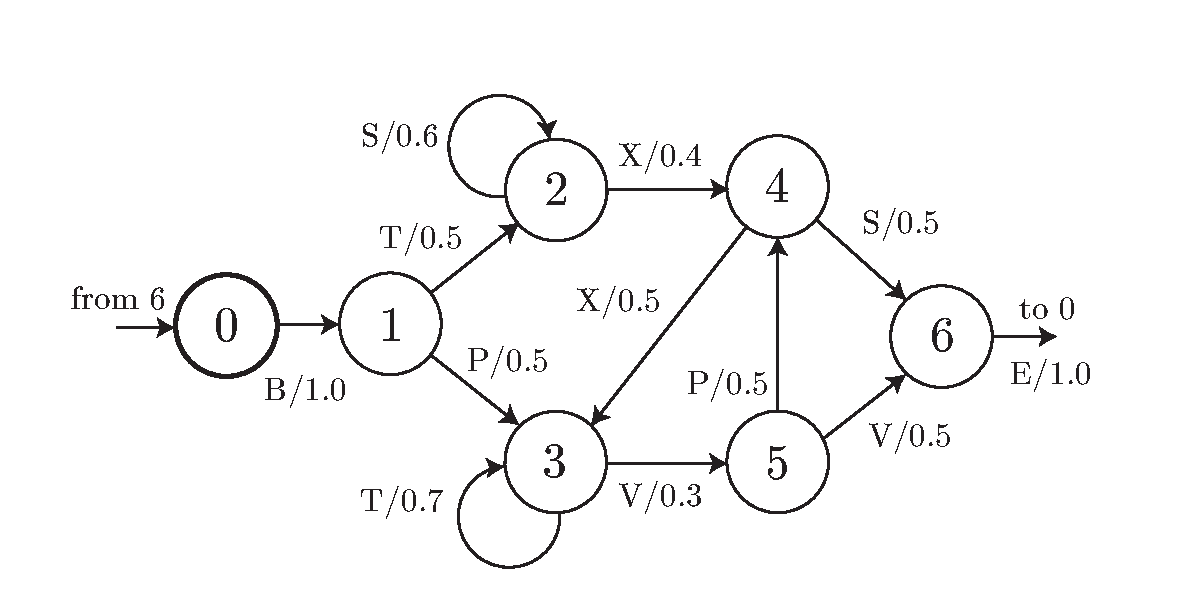
\includegraphics[scale=0.32]{reber.pdf}\label{subfig:reber}}  \hspace{-1.25cm} 
\subfigure[Feldman]{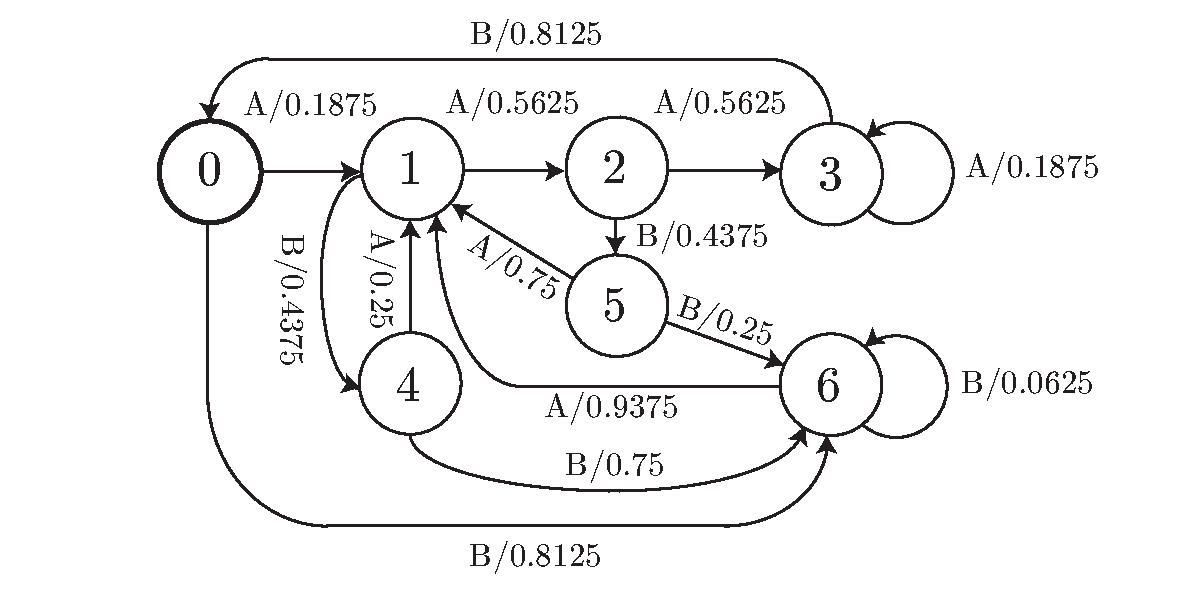
\includegraphics[scale=0.32]{feldman.pdf}\label{subfig:feldman}} \\
\subfigure[Posterior marginal PDIA state cardinality distribution]{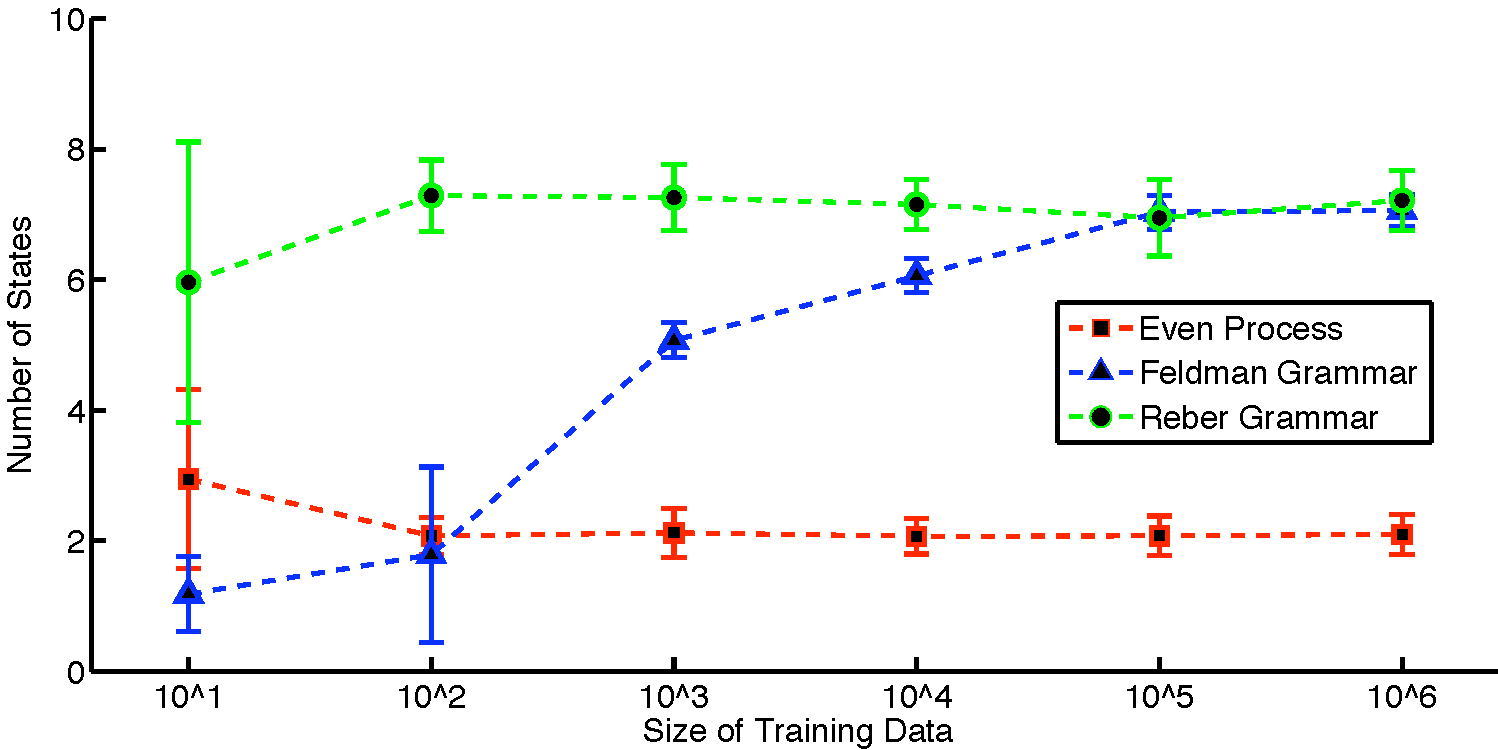
\includegraphics[scale=0.3]{results/syntheticResults.pdf}\label{subfig:posterior}}
\label{fig:synthetic_grammar_and_synth_results}
\caption{Three synthetic PDFAs: \subref{subfig:even} even process, \subref{subfig:reber} Reber grammar, \subref{subfig:feldman} Feldman grammar.  \subref{subfig:posterior} posterior mean and standard deviation of number of states discovered during PDIA inference for varying amounts of data generated by each of the synthetic PDFAs.  PDIA inference discovers PDFAs with the correct number of states}
\end{figure}

%\section{Related Work}

Despite a wealth of research on both the theory and practice of learning PDFAs, the work presented here is, to our knowledge, the first algorithm to generate samples from a posterior over automata rather than returning a deterministic estimate.  Prior work has focused on greedy algorithms, which work by either merging or splitting elements of $Q$ according to some statistical test.  Theoretical work has shown that PDFAs are both identifiable in the limit and, with a few restrictions on the model class\footnote{A polynomial number of states in the true automata, a minimum divergence between the distribution over strings that follow two states, and a polynomial bound on the probability of generating strings above a certain length}, are also PAC-learnable\footnote{A model class is said to be {\em PAC-learnable} if there is an algorithm that will return, in time polynomial in $\frac{1}{\delta}$,$\frac{1}{\epsilon}$ and $|D|$, an estimate within an accuracy $\epsilon$ of the true model from $|D|$ examples with probability $1-\delta$.} using KL divergence between automata as a measure of accuracy.

\subsection{State Merging Algorithms}
A variety of algorithms work by starting with the trivial automata built from the prefix tree of the data, and generalizes by merging states that pass a similarity test.  Merging two states is not trivial: if $\delta(q_1,s_j) \ne \delta(q_2,s_j)$, then merging $q_1$ and $q_2$ will produce a state with nondeterministic transitions.  This is avoided by recursively merging the states $\delta_{1j}$ and $\delta_{2j}$ until the resulting automata is deterministic.  The result is a {\em quotient automata} of the original.  One of the earliest algorithms to use this method is ALERGIA \cite{Oncina1994}, which uses a test based on the Hoeffding bound to decide whether to merge states, and was proven to converge to the true automata in the limit of infinite data.

Later algorithms have mostly focused on improving the state merging test.  MDI uses a test based on the KL divergence between automata, and penalizes automata with many states.  Thus it can be interpreted as a greedy maximum posterior estimator with a minimum description length prior.  Empirically, it has better predictive performance than ALERGIA on natural language data.

\cite{Clark2004} presented a state-merging algorithm for cyclic PDFAs that is PAC-learnable given very few restrictions on the model class.  While the emphasis was on theoretical rather than empirical performance, it was also shown to work well from small data.

\subsection{State Splitting Algorithms}

State splitting algorithms, by contrast, start with the most general single-state automata and become more selective by adding more states.  \cite{Ron1995} learned a variable-order Markov model using a state-splitting algorithm, where a state corresponding to a string suffix was split into states corresponding to longer suffixes according to some test (*hm...all this "according to some test" is getting redundant.  Might want to rephrase this*).  Splitting might occasionally produce nondeterministic transitions.  For example, after splitting the context $01$ into $001$ and $101$, the context $0$ and symbol $1$ might transition to either one, unless the context $0$ is also split into $10$ and $00$, but these probabilistic suffix trees could be mapped onto PDFAs after learning.

CSSR \cite{Shalizi2004} took a similar approach, but with a model class that contains all PDFAs.  Their philosophical motivation, similar to ours, is to learn the minimal sufficient statistics for predicting the future given the past.  Given a stationary sequence with infinitely long past and future, those statistics form a PDFA, which they call a {\em causal state machine}.  Each state is a set of suffixes, rather than a single suffix, which means the model class includes all PDFAs.  If the predictive distribution for a suffix passes a Kolmogorov-Smirnov test, that state is split in two and suffixes in the original state are divided.  Nondeterministic transitions are removed recursively by backing up to the states preceding a split state and splitting in the natural way, much like the reverse of how states are merged when forming quotient automata.


% !TEX root = main.tex
\section{Experiments and Results}
\label{sec:results}
\comment{

\begin{table}[t]
    \begin{center}
    \setlength{\tabcolsep}{1.3mm}
\begin{tabular}{r|cccccccccc}
\hline
& {\bf PDIA } & PDIA-MAP &  HMM-EM & bigram& trigram & 4-gram & 5-gram & 6-gram & SSM \\
\hline
AIWS & 2.36 & 2.45 &  2.98 & 3.28 & 2.69 & 2.36 & 2.26 & 2.23 & 2.26 \\
AIWS & 373.3 & 379 & 52 & 28 & 382 & 2023 & 5592 & 10,838 & 19,358 \\
\hline
\hline
AIWL & 2.03 & 2.05 &  2.98 & 3.24 & 2.52& 2.02 & 1.81 & 1.73 & 1.70 \\
AIWL & 1,231.6 & 1,247 &  52 & 28 & 444 & 3,249 & 12,324 & 31,990 & 177,232 \\
\hline
\hline
DNA & 1.89 & 1.90 &  1.91 & 1.92* & 1.91 & 1.90 & 1.90 & 1.90 & 1.83 \\
DNA & 61.3 & 54 & 46.2* &  5 & 21 & 85 & 341 & 1,365 & 314,166 \\
\hline
\end{tabular}
\end{center}
\caption[Short]{Benchmark performance of PDIA inference algorithms versus standard sequence models.}
\label{table:results}
\end{table}


\begin{table}[t]
    \begin{center}
    \setlength{\tabcolsep}{1.3mm}
\begin{tabular}{r|cccccccccc}
\hline
& {\bf PDIA } & PDIA-MAP &  HMM & bigram& trigram & 4-gram & 5-gram & 6-gram & SSM \\
\hline
AIWS & 2.362 & 2.448 &  2.98 & 3.275 & 2.687 & 2.358 & 2.263 & 2.230 & 2.257 \\
AIWS & 373.3 & 379 & 52 & 28 & 382 & 2023 & 5592 & 10838 & 19358 \\
\hline
\hline
AIWL & 2.027 & 2.047 &  2.98 & ? & 2.517 & 2.018 & 1.811 & 1.729 & 1.697 \\
AIWL & 1231.6 & 1247 &  52 & 28 & 444 & 3249 & 12324 & 31990 & 177232 \\
\hline
\hline
DNA & 1.894 & 1.896 &  1.909 & 1.915* & 1.906 & 1.903 & 1.898 & 1.895 & 1.832 \\
DNA & 61.3 & 54 & 46.2* &  5 & 21 & 85 & 341 & 1365 & 314166 \\
\hline
\end{tabular}
\end{center}
\caption[Short]{Benchmark performance of PDIA inference algorithms versus standard sequence models.}
\label{table:results}
\end{table}
}


\begin{table}[t]
    \begin{center}
    \setlength{\tabcolsep}{1.3mm}
\begin{tabular}{r|cccccccccc}
\hline
& PDIA  & PDIA-MAP &  HMM-EM & bigram& trigram & 4-gram & 5-gram & 6-gram & SSM \\
\hline
AIWS & 5.13 & 5.46 &  7.89 & 9.71 & 6.45 & 5.13 & 4.80 & 4.69 & 4.78 \\
AIWS & 373.3 & 379 & 52 & 28 & 382 & 2023 & 5592 & 10,838 & 19,358 \\
\hline
\hline
AIWL & 4.08 & 4.13 &  7.89 & 9.45 & 5.72 & 4.05 & 3.51 & 3.32 & 3.24 \\
AIWL & 1,231.6 & 1,247 &  52 & 28 & 444 & 3,249 & 12,324 & 31,990 & 177,232 \\
\hline
\hline
DNA & 3.72 & 3.72 &  3.76 & 1.92* & 3.75 & 3.74 & 3.73 & 3.72 & 3.56 \\
DNA & 61.3 & 54 & 46.2* &  5 & 21 & 85 & 341 & 1,365 & 314,166 \\
\hline
\end{tabular}
\end{center}
\caption[Short]{Benchmark performance of PDIA inference algorithms versus standard sequence models.}
\label{table:results}
\end{table}

\begin{figure}[htbp]
\centering
\subfigure[DNA HMM EM Baseline]{\label{fig:dna_hmm}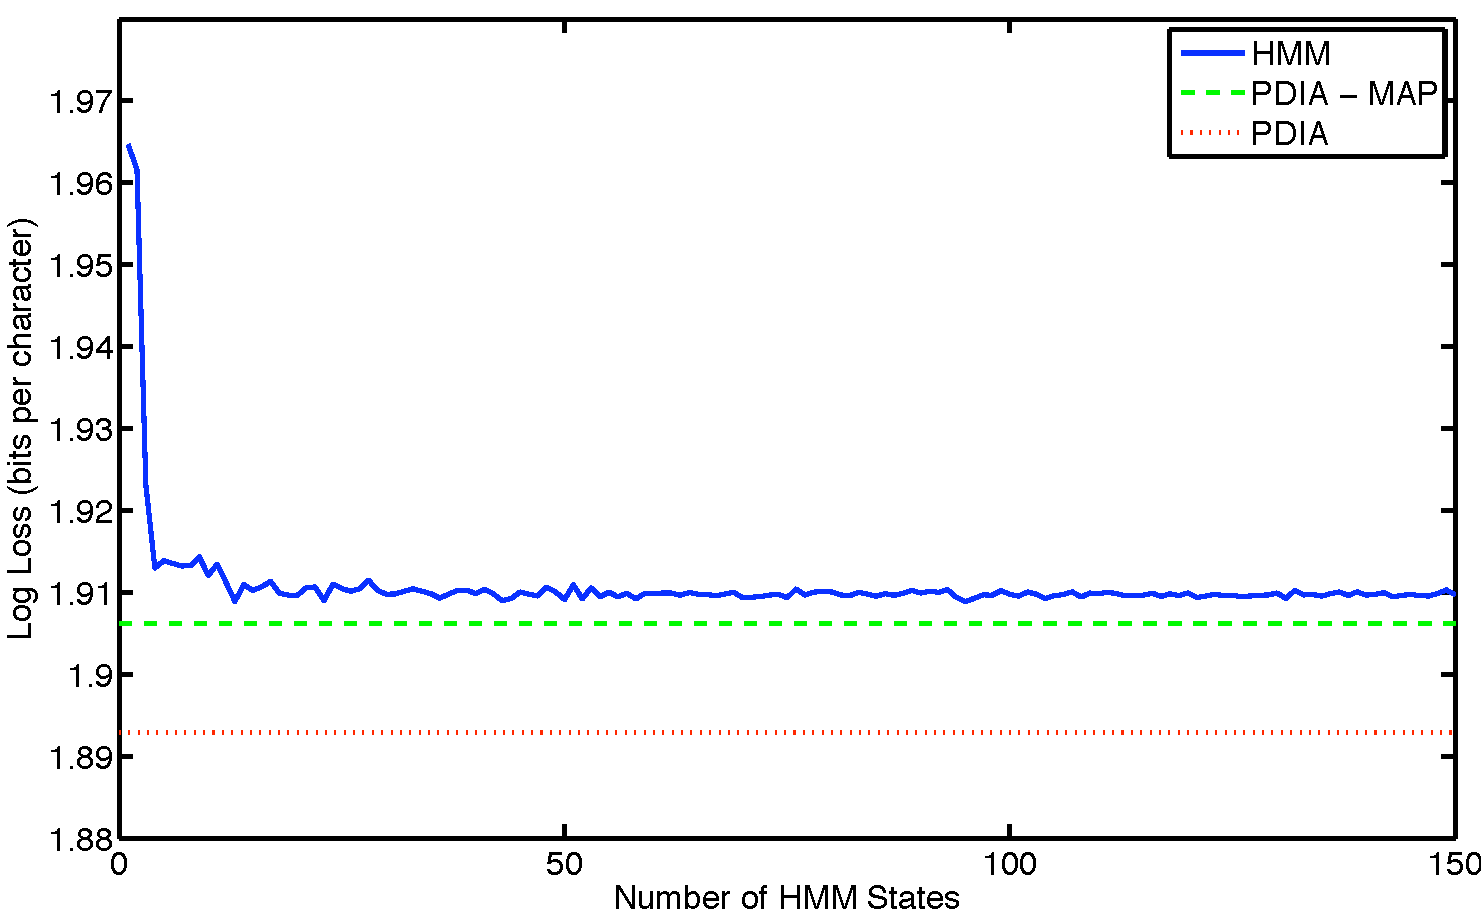
\includegraphics[width=.3\textwidth]{results/dna_hmm}}
\subfigure[DNA sampler trace]{\label{fig:dna_sampler}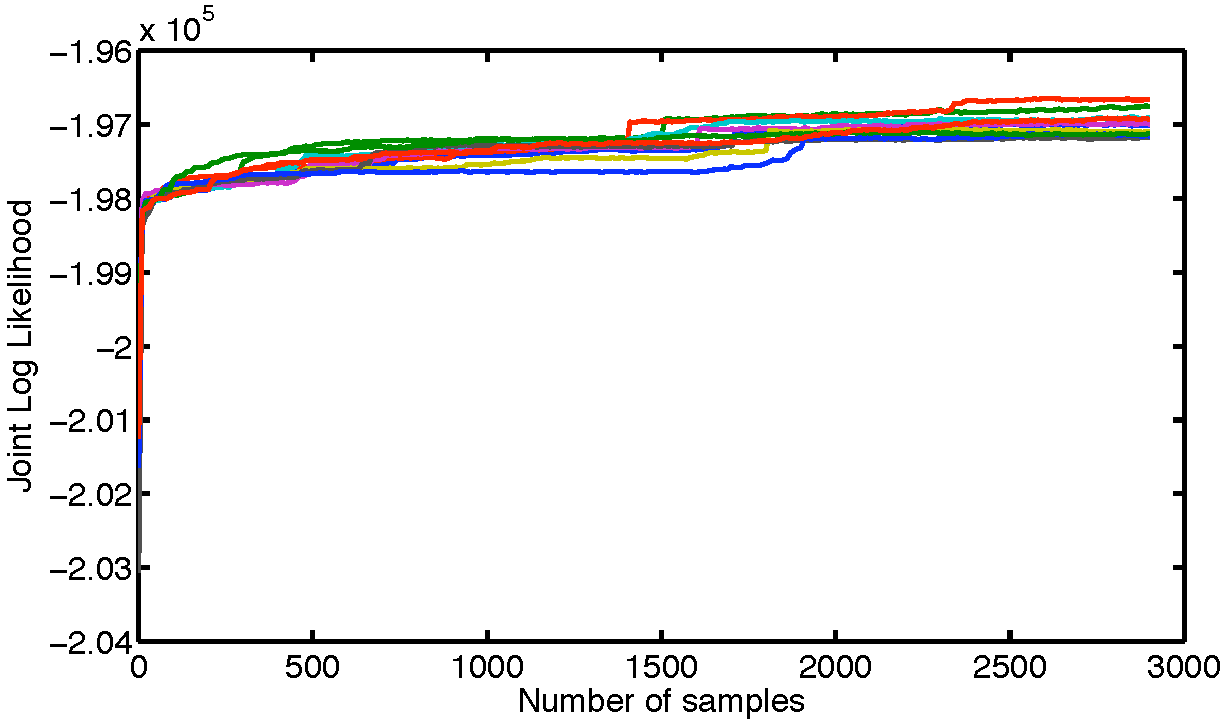
\includegraphics[width=.3\textwidth]{results/dna_sampler}}
\subfigure[DNA number of states]{\label{fig:dna_numstates}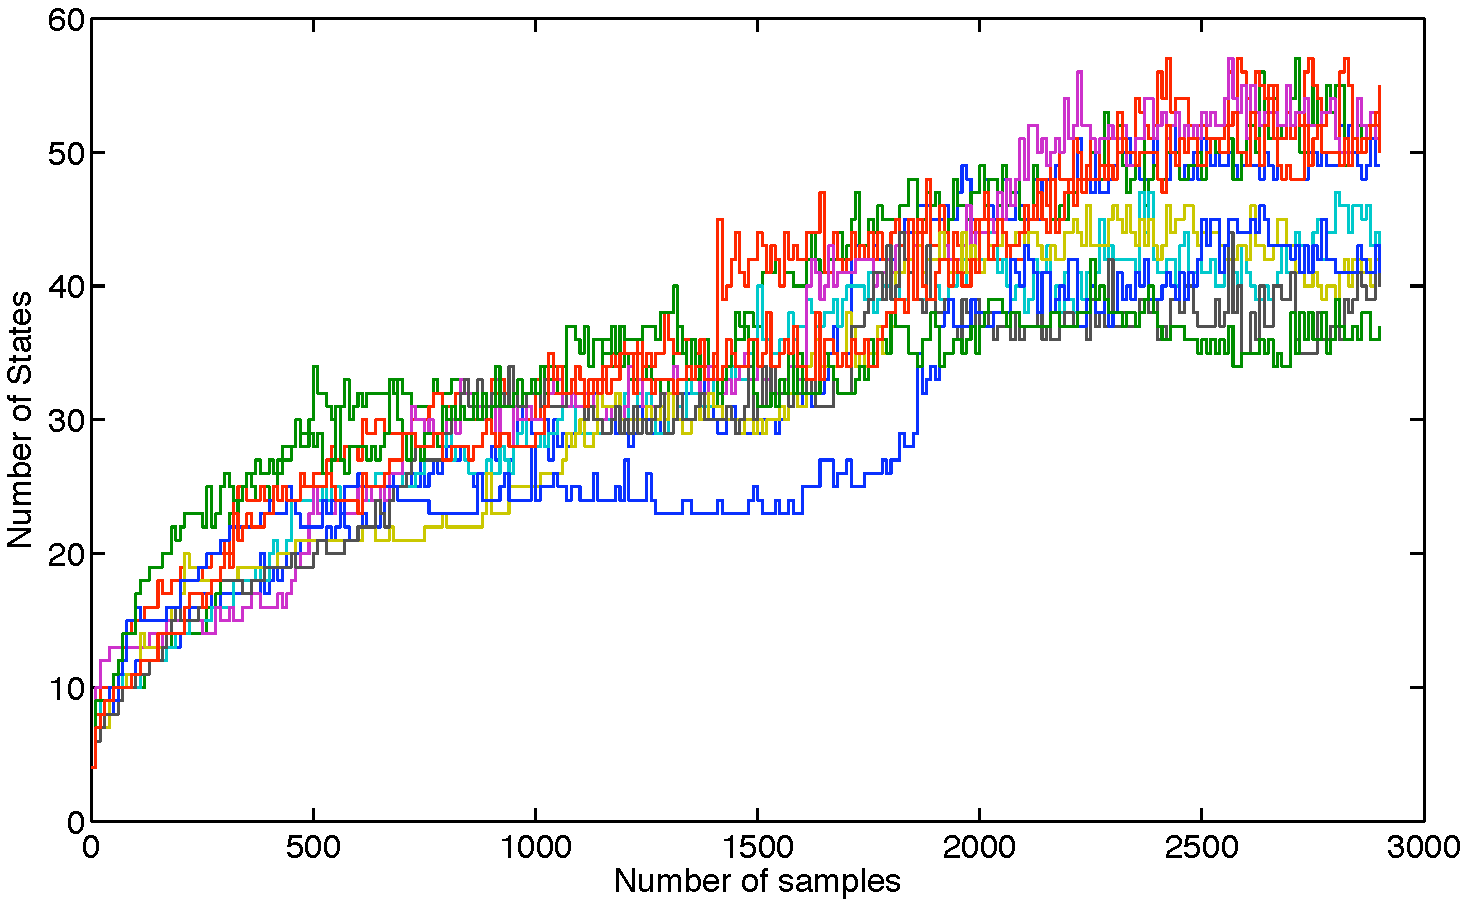
\includegraphics[width=.3\textwidth]{results/dna_numstates}}\\
\subfigure[AIW HMM EM Baseline]{\label{fig:aiw_small_hmm}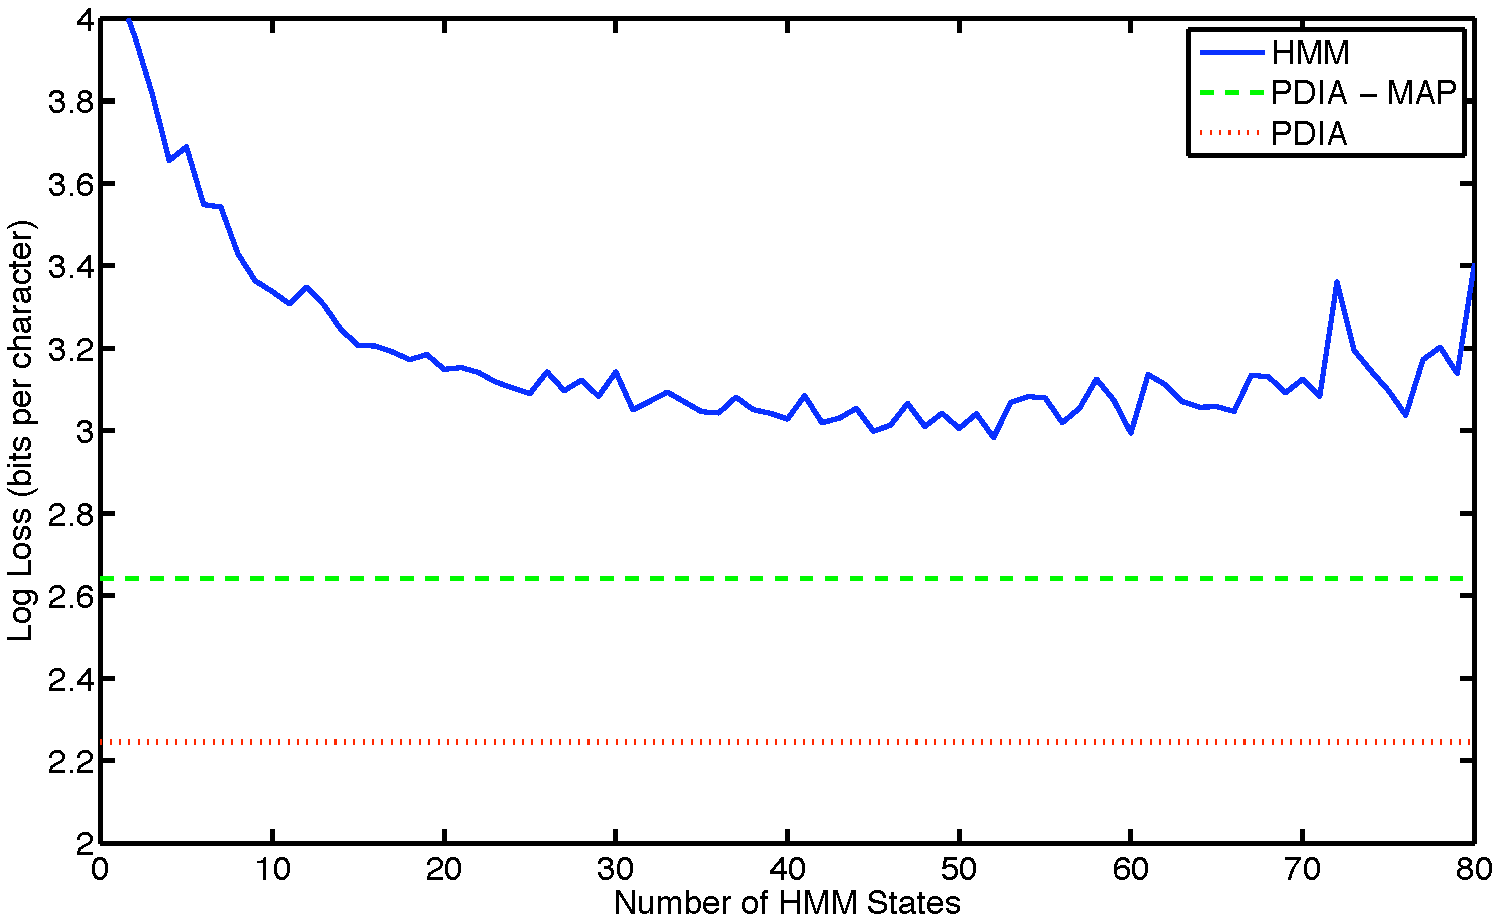
\includegraphics[width=.3\textwidth]{results/aiw_small_hmm}}
\subfigure[AIW sampler trace]{\label{fig:aiw_small_sampler}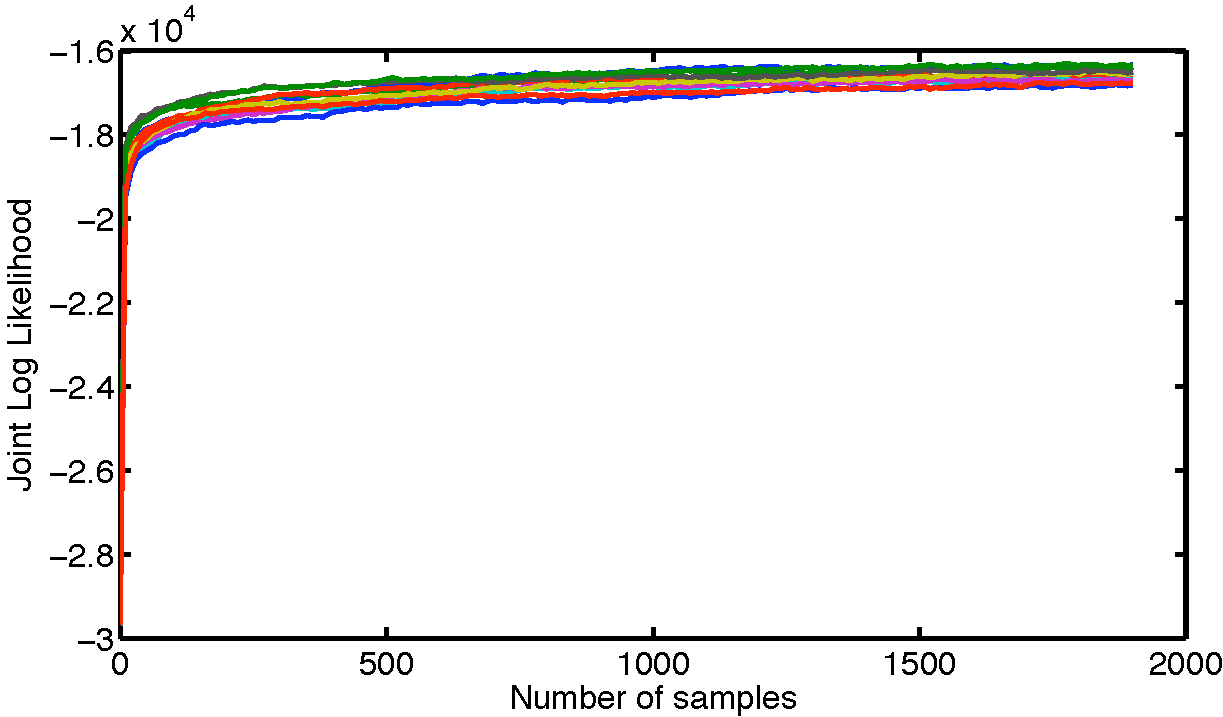
\includegraphics[width=.3\textwidth]{results/aiw_small_sampler}}
\subfigure[AIW number of states]{\label{fig:aiw_small_numstates}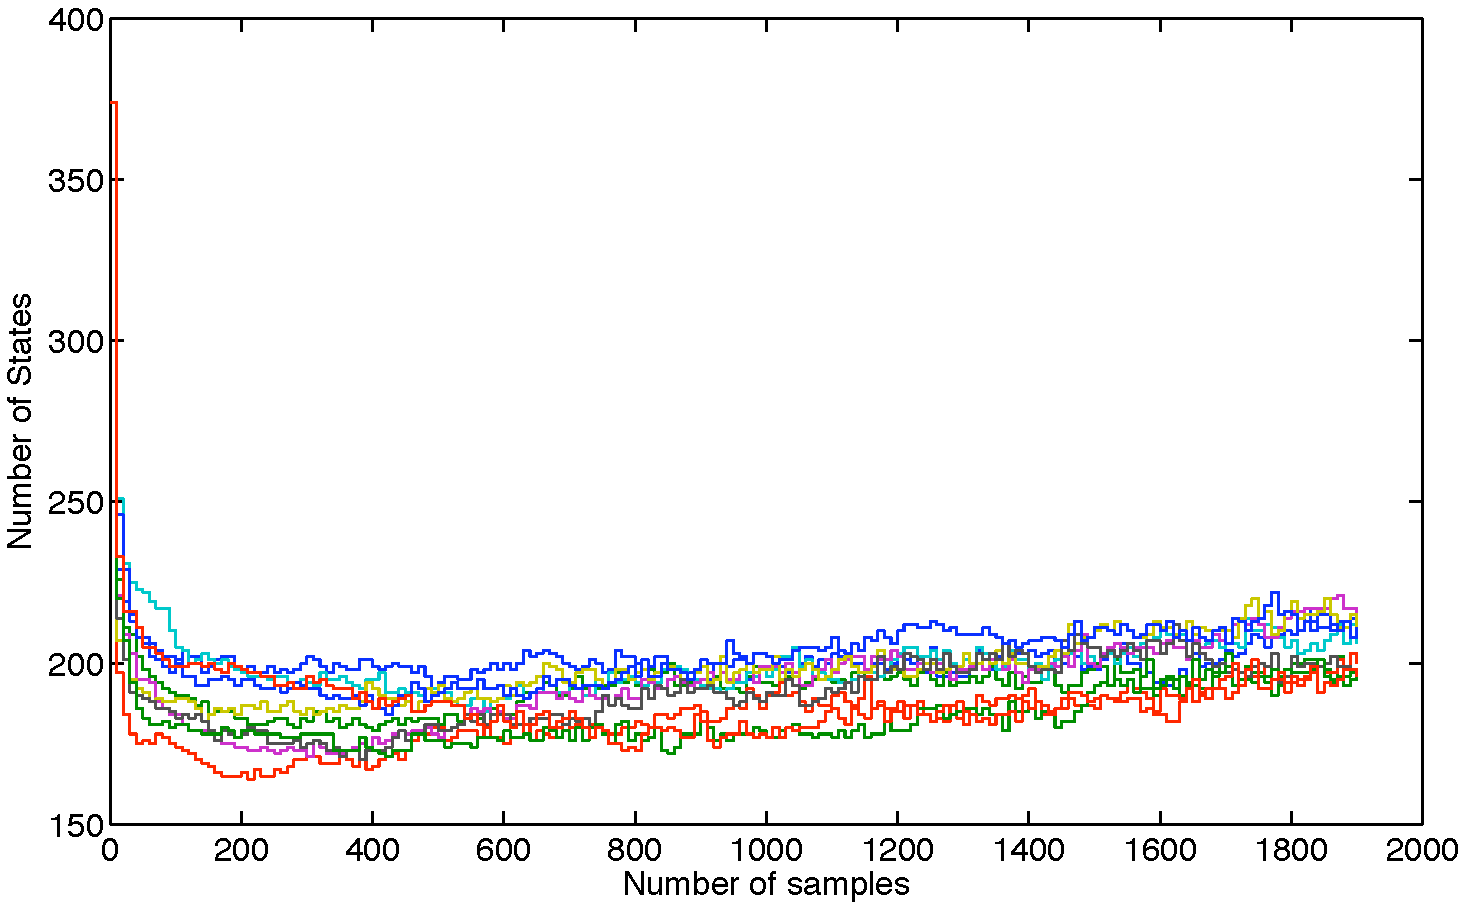
\includegraphics[width=.3\textwidth]{results/aiw_small_numstates}}
\caption{}
\label{fig:aiw_and_dna_all_figs}
\end{figure}

To evaluate our PDIA inference approach we used it to do discrete sequence prediction and compared its performance to other approaches to the same.  We trained our model and others on two datasets: a character sequence from Alice in Wonderland and a short sequence of mouse DNA.  The Alice in Wonderland dataset was preprocessed to remove all characters but letters and spaces, shift all letters from upper case to lower case, and split along sentence dividers to yield a 27-character alphabet (a-z and space) and 1639 sentences with a total of 132794 characters.  We used the first 1200 sentences (100210 characters) to train the models and the rest to test.  \comment{For some experiments we also used a smaller subset of Alice in Wonderland consisting of 100 randomly chosen training sentences (9986 characters) and 50 random test sentences (3891 characters).}  The mouse DNA dataset consisted of a fragment of chromosome 2 with 194173 base pairs, which we treated as a single unbroken string.  We used the first 150000 base pairs for training and the rest for testing.  For Alice in Wonderland, the state of the PDIA model was always set to $q_0$ at the start of each sentence.  For DNA, the state of the PDIA model at the start of the test data was set to the last state of the model after accepting the training data.  We placed Gamma(1,1) priors over $\alpha$,$\beta$ and $\gamma$ and set $\lambda=.001.$

We evaluated the performance of the learned models by calculating the average per character predictive perplexity of the test data.  For training data $x_{1:T}$, test data $y_{1:T'}$ this is given by $2^{-\frac{1}{T'}\log_2\, P(y_{1:T'}|x_{1:T})}$.  It is an average measure of the uncertainty the model has about what character comes next in the sequence given the sequence up to that point. It is at most $|\Sigma|$, which for DNA is 4 and for text is 27.  We evaluated the probability of the test data incrementally, integrating test observations into the model in the standard Bayesian way, and averaged each predictive probability $P(y_{1:T'}|x_{1:T}) =  \prod_{i = 1}^{T'} \int P(y_i|y_{1:i-1},x_{1:T},\delta)P(\delta|y_{1:i-1},x_{1:T})d\delta \approx \frac{1}{L}\prod_{i = 1}^{T'} \sum_{\ell = 1}^{L} P(y_i|y_{1:i-1},x_{1:T},\delta_\ell)$ where $\delta_\ell \sim P(\delta|y_{1:i-1},x_{1:T})$.  %In addition to averaging over multiple $\delta_\ell$, we also evaluated the log loss for each $\delta_\ell$ by itself to find the single model with the best generalization performance, which we call $\delta_{MAP}$.

Test results are shown in Table~\ref{table:results}.  
For the smoothed $n$-gram models, we report average perplexity results for hierarchical Pitman-Yor process (HPYP) \cite{Teh2006} models of varying Markov order (1 through 5 notated as bigram through 6-gram) burned in for one hundred samples and averaged over 1000.  While the PDIA averages over a  class of models that includes finite order Markov models as a subset, the states in HPYP are identifiable which means that hierarchical smoothing of the per-state emission distributions is possible.  In the PDIA model the states are not identifiable and no easily defined hierarchy of contextual specificity exists on which hierarchical smoothing could be implemented.  


We show the performance of the incremental variant of the sequence memoizer (SM) \cite{Gasthaus2010}, which is the limit of an $n$-gram as $n\rightarrow\infty$.

For a baseline result to compare our model against, we used two models: a hidden Markov model (HMM) and a smoothed n-gram model.  We used Kevin Murphy's HMM toolbox \cite{Murphy} and trained the HMM using expectation-maximization (EM).  We found the best number of hidden states by cross-validation on the same test data used for the PDIA.  The log loss and optimal number of states are given in Table \ref{table:results}, and plots showing the generalization performance across a range of model sizes relative to PDIA performance is given in Figures \ref{fig:dna_hmm} and \ref{fig:aiw_small_hmm}.  

We found that both the MAP PDIA and the average over PDIA generalize better than the HMM.  To test the possibility that better generalization was due to smoothing of the PDIA emission probability by $\beta$, we took samples from the PDIA, fixed $\beta$ to be very near 0, and ran the MCMC sampler as before.  We found that neither the average number of states nor the generalization performance was significantly affected.

In general it seems that posterior samples from the PDIA achieve competitive generalization performance on natural language and DNA compared to hidden Markov models and n-gram models.  Averaging predictive probability over multiple samples leads to better generalization than a single sampled model.  Both a single sample and multiple samples generalize better than the best EM-trained HMM.  On natural language, the learned PDIA has more states than the optimal number of states for an HMM found by cross-validation.  The improved generalization is not due to smoothing the emission distribution.  Compared to smoothed n-gram models, the PDIA performs competitively even though there is no backing off to more general contexts.


%Even for a single sampled transition matrix $\delta_\ell$, there may be symbols $y_t$ which have not been emitted from the state $\q_t$ in the training data, and thus $\delta_\ell(\q_t,y_t)$ is not known.  In this case we sampled a new element of the transition matrix according to the CRF, as described in \ref{model}.  In the same way that we averaged the predictive probability of each character over multiple $\delta_\ell$, we averaged the probability of a character given a single $\delta_\ell$ over multiple sampled values of $\delta_\ell(\q_t,y_t)$.





% !TEX root = main.tex
\section{Discussion}
\label{section_discussion}

Things to consider: 

1) Scaling to phrases.
2) Making the spelling correction parameterization context dependent.


http://people.csail.mit.edu/jrg/2006/hsu\_emnlp06.pdf
http://www.panl10n.net/english/final%20reports/pdf%20files/Bangladesh/BAN08.pdf
http://www.coli.uni-saarland.de/~thorsten/tnt/

%\subsubsection*{Acknowledgments}

%\subsubsection*{References}
\begin{small}
\bibliographystyle{plainnat}
\bibliography{../../uber} 
%\input{modrefs}
\end{small}
\end{document}
